%%%%%%%%%%%%%%%%
% Final Report for PHAS3441%
%%%%%%%%%%%%%%%%

%----------------------------------------------------------------------------------------
%	PACKAGES AND OTHER DOCUMENT CONFIGURATIONS
%----------------------------------------------------------------------------------------
\documentclass[11pt, english, singlespacing, headsepline,]{FinalReport} 
\usepackage[utf8]{inputenc}
\usepackage[T1]{fontenc}
\usepackage{times} % font
\usepackage[backend=bibtex,style=authoryear,natbib=true]{biblatex} % citation style, change if needed
\addbibresource{references.bib} % The filename of the bibliography (see folder)
\usepackage[autostyle=true]{csquotes} % Required to generate language-dependent quotes in the bibliography

%----------------------------------------------------------------------------------------
%	MARGIN SETTINGS
%----------------------------------------------------------------------------------------

\geometry{
	paper=a4paper, 
	inner=2.3cm, % Inner margin
	outer=3.8cm, % Outer margin
	bindingoffset=2cm, % Binding offset
	top=1.5cm, % Top margin
	bottom=1.5cm, % Bottom margin
	%showframe,% show how the type block is set on the page
}

%----------------------------------------------------------------------------------------
%	REPORT INFORMATION
%----------------------------------------------------------------------------------------

\thesistitle{Annihilation Gamma Ray Laser \\ A Feasibility Report } 
\supervisor{Dr. David \textsc{Cassidy}}
\degree{UCL MSci Physics Program} 
\author{Andreas Angelis \textsc{Christou}, Edward \textsc{Mercer}, Iarom \textsc{Madden}, Gabriela \textsc{May Lagunes}, Mark \textsc{Jenie}, Omree \textsc{Naim}, Poonam \textsc{Sodha}, Sussie \textsc{Sujeeporn}}
\subject{Physics} 
\keywords{Annihilation, Gamma Ray, Laser} % Keywords for your thesis, this is not currently used anywhere in the template, print it elsewhere with \keywordnames
\university{\href{http://www.ucl.ac.uk/}{University College London}} 
\department{\href{www.phys.ucl.ac.uk/}{Physics and Astronomy}} 
\group{\href{http://www.ucl.ac.uk/prospective-students/undergraduate/degrees/physics-msci/}{Group Project 8}} 
\faculty{\href{https://www.ucl.ac.uk/mathematical-physical-sciences}{UCL Faculty of Mathematial and Physical Sciences}} 
\hypersetup{pdftitle=\ttitle} % Set the PDF's title to your title
\hypersetup{pdfauthor=\authorname} % Set the PDF's author to your name
\hypersetup{pdfkeywords=\keywordnames} % Set the PDF's keywords to your keywords

\begin{document}

\frontmatter % Use roman page numbering style (i, ii, iii, iv...) for the pre-content pages

\pagestyle{plain} % Default to the plain heading style until the thesis style is called for the body content

%----------------------------------------------------------------------------------------
%	TITLE PAGE
%----------------------------------------------------------------------------------------

\begin{titlepage}
\begin{center}

{\scshape\LARGE \univname\par}\vspace{1.5cm} % University name
\textsc{\Large PHAS3441: Group Project Final Report}\\[0.5cm] 

\HRule \\[0.4cm] % Horizontal line
{\huge \bfseries \ttitle\par}\vspace{0.4cm} % Thesis title
\HRule \\[1.5cm] % Horizontal line

\begin{minipage}[t]{0.4\textwidth}
\begin{flushleft} \large
\emph{Team Membesr}\\
\href{http://www.ucl.ac.uk}{\authorname} % Author name - remove the \href bracket to remove the link
\end{flushleft}
\end{minipage}
\begin{minipage}[t]{0.4\textwidth}
\begin{flushright} \large
\emph{Board Member} \\
\href{https://iris.ucl.ac.uk/iris/browse/profile?upi=DBCAS57}{\supname} % Supervisor name
\end{flushright}
\end{minipage}\\[3cm]
 
\large \textit{A report submitted in fulfillment of the requirements\\ for the module PHAS3441 of \degreename}\\[0.3cm] % University requirement text
\textit{sent by}\\[0.4cm]
\groupname\\\deptname\\[2cm] % Research group name and department name
 
\textit{March the 21st, 2016}\\[4cm] % Date
%\includegraphics{Logo} % University/department logo - uncomment to place it
 
\vfill
\end{center}
\end{titlepage}

%----------------------------------------------------------------------------------------
%	DECLARATION PAGE
%----------------------------------------------------------------------------------------

\begin{declaration}
\addchaptertocentry{\authorshipname}

\noindent We, \authorname, declare that this report titled, 'Annihilation Gamma Ray Laser: A Feasibility Report' and the work presented in it are our own. We confirm that:

\begin{itemize} 
 \item This work was done wholly or mainly while the completion of an undergraduate degree at this University.
 \item Where we have consulted the published work of others, this is always clearly attributed.
 \item Where we have quoted from the work of others, the source is always given. With the exception of such quotations, this thesis is entirely our own work.
 \item We have acknowledged all main sources of help.
\end{itemize}
 
\noindent Signed:\\
\rule[0.5em]{25em}{0.5pt}\\ % This prints a line for the signature
\rule[0.5em]{25em}{0.5pt}\\
\rule[0.5em]{25em}{0.5pt}\\
\rule[0.5em]{25em}{0.5pt}\\
\rule[0.5em]{25em}{0.5pt}\\
\rule[0.5em]{25em}{0.5pt}\\
\rule[0.5em]{25em}{0.5pt}\\
\rule[0.5em]{25em}{0.5pt}\\
 
\noindent Date:\\
\rule[0.5em]{25em}{0.5pt} % This prints a line to write the date
\end{declaration}

\cleardoublepage

%----------------------------------------------------------------------------------------
%	RESPONSIBILITY ALLOCATION PAGE
%----------------------------------------------------------------------------------------

\begin{responsibility}
\addchaptertocentry{\responsibilityname}

\noindent The challenges identified during this project were divided per subject. These were distributed as follows. However, it is worth noting that every member of the team was involved in the general development and decision making process of the project. 

\begin{itemize} 
 \item Positron and Positronium Production and Storage: Mark Jenei, Poonam Sodha and Iarom Madden.
 \item Bose-Einstein Condensate: Gabriela May Lagunes, Omree Naim and Sujeeporn Tuntipong.
 \item Laser Engineering and Gamma-Ray Optics: Andreas Angelis Christou and Edward Mercer.
 \item An Alternative Method: Andreas Angelis Christou and Omree Naim.
 \item Applications, Manufacturing Cost and Production Time Scale: Andreas Angelis Christou, Gabriela May Lagunes and Edward Mercer.
\end{itemize}
 
\noindent The general administration of the project and the communication process with the Board and other groups was coordinated by Gabriela May-Lagunes and Poonam Sodha.\\
 
\end{responsibility}

\cleardoublepage

%----------------------------------------------------------------------------------------
%	QUOTATION PAGE
%----------------------------------------------------------------------------------------

\vspace*{0.2\textheight}

\noindent\enquote{\itshape There is an extremely powerful force that, so far, science has not found a formal explanation to. It is a force that includes and governs all others, and even behind any phonomenon operating in the Universe and has not yet been identified by us. The universal force is Love.}\bigbreak

\hfill Albert Einstein

%----------------------------------------------------------------------------------------
%	EXECUTIVE SUMMARY 
%----------------------------------------------------------------------------------------

\begin{abstract}

\addchaptertocentry{\abstractname} % Add the abstract to the table of contents

The aim of this report is to determine the feasibility of the production of an annihilation ? ray laser via the use of Positronium by summarising any and all technological challenges currently present that are obstructing the construction of said device. A tangential aim is to also summarise any alternatives to the primary schema that will be investigated to develop the annihilation laser. In addition to this, a secondary aim was to conduct a costing study to provide economic context to the production of the laser, along with an idea of the length of time that would be required to produce the laser. The final aim of the report was to provide modern processes in which an annihilation ? ray laser would have been specifically useful.
In order to carry out the first aim of the production of the laser, a set of objectives had to be met. First and foremost research needed to be conducted to determine a method suitable for the creation and storage of a large number of Positrons (on the order of ~1017). This research also included the investigation of any health and safety requirements that needed to be met to deal with the issue of radiation doses presented by the Positron production (e.g. investigating the development of shielding to attenuate Bremsstrahlung radiation) . Upon completion of this objective, the next objective uses the aforementioned Positrons to create the  Positronium in a large enough density to allow for condensation (or at a low enough temperature). This objective required the investigation into the required conditions for Bose-Einstein condensation of Positronium (e.g. critical density, critical temperature etc). Following the research into the condensation of the Positronium into a Bose-Einstein condensate state, further research then had to be conducted to determine a method that could be used to detect that the Positronium had actually attained this exotic state of matter, assuming that the detection of the transition  is physically possible. Once detection of the BEC formation is complete, the next objective to be met is to research a scheme that would allow spin flipping of the Positronium forming the BEC that would then cause stimulated annihilation to take place. This stimulated annihilation essentially forms the basis of the laser and from here the physics becomes more theoretical and lacks experimental support. The next objective was to conduct research into the area of ? ray optics which is necessary for the following two reasons; firstly the annihilation of the BEC would cause emission of ? rays in random directions thereby requiring a reflection or refraction mechanism to be in place to prevent the loss of ~50\% of the energy produced in annihilation, and secondly a focussing mechanism would also need to be developed to focus the ? rays into a coherent beam which could then be used by the consumer as required. A secondary objective of the ? ray optics section is the requirement of suitable shielding to be produced in conjunction with the laser to prevent the irradiation of any users by any stray ? rays that could potentially be emitted from the laser. The final objective is to investigate the field of ? ray detectors to ascertain if there is a detector of suitable durability that could be used to measure the output power of the ? ray laser. These objectives allowed for completion of the first aim.
The laser production aim also required calculations to be made to ensure that the schema that we had chosen to use would guarantee that a kilojoule laser would  be produced. These calculations included, but were not limited to; determining the upper limit to the amount of Positronium that we could produce in a beam based on the most active Positron source currently available, the calculation of the critical densities and temperature for the condensation of Positronium etc. These calculations were carried out  after the previously discussed was complete to ensure that the most efficient methods were used throughout rather than using older processes that have then been superseded by modern processes. There were some cases where results may not be presented due to a lack of mathematical background required to carry out the rigorous calculations. A supplementary objective was also the potential computational simulation of the Positron and Positronium beams using SIMION. This would have been done to aid in the providing of precise results that would aid in the determination of the feasibility of this schema in creating the laser.  

The aim of producing a costing report was met by successively determining the cost of current and contemporary experiments for each applicable section, and also by investigating if there have been any reductions in costs of experimental components to date (e.g. reduction in the cost Gallium which would be used for Positron production). Any components currently in development also needed to be investigated (e.g. the Silicon prisms in the ? ray optics section), and if costs were unavailable then they were approximated via usage of any public knowledge on the research grants provided to studies into said developing component. A Gantt chart was also produced by estimating relative time scales for completion of each section previously discussed. This required the investigation into the length of time taken to complete any previous experiments that contained components that would be used to produce the laser. In the case of areas that are still in development this was again estimated based on peer reviewed papers which provided time scales for the production of the necessary components. These two objectives allowed for the second aim of the report to be met.
In order to meet the final aim of the report, a discussion took place to determine the consensus of the group on what fields would find the most use of an annihilation ? ray laser. Once a consensus had been reached any use of lasers in these areas was then specifically researched to determine if a ? ray laser may have been more appropriate for the same task. In terms of applications in which an annihilation ? ray laser would be a definitive requirement, previously used papers were used to determine if they were in the process of developing a ? ray laser for a specific usage that only the laser was capable of meeting. Research was also conducted into current laser usages to determine if there were tasks that modern lasers were not capable of carrying out due to power limitations. If so then these tasks may be tasks that only a ? ray laser would be capable of. Also any tasks requiring a very high degree of precision were investigated as these would be tasks that only a ? ray laser would be capable of conducting due to the small wavelength of the photons that the beam consists of. 

The final outcome of this project is the determination that the production of an annihilation ? ray laser using the Bose-Einstein condensation of Positronium is not possible with the currently available technology. The main reasons for this are covered in detail on page XX in the Unresolved Problems section. However, this report also presents a possible alternative method that may be feasible with current technology as it eliminates the main issue presented in this report which is the generation of a Bose-Einstein condensate of Positronium which in turn is an issue caused by the inability to produce Positrons at a sufficient density within the beam to ensure the critical density of Positronium is then reached.

\end{abstract}

%----------------------------------------------------------------------------------------
%	ACKNOWLEDGEMENTS
%----------------------------------------------------------------------------------------

\begin{acknowledgements}
\addchaptertocentry{\acknowledgementname} % Add the acknowledgements to the table of contents

The members of the Group Project 8 would like to thank Dr. David Cassidy for his support and advice during the production of the this document. Special thanks to Dr. Paul Bartlett and Prof. Allen Mills for their comments and discussions during the development of the project. Finally, we thank the department for the opportunity of working in this subject.  

\end{acknowledgements}

%----------------------------------------------------------------------------------------
%	LIST OF CONTENTS/FIGURES/TABLES PAGES
%----------------------------------------------------------------------------------------

\tableofcontents % Prints the main table of contents

%\listoffigures % Prints the list of figures

%\listoftables % Prints the list of tables

%----------------------------------------------------------------------------------------
%	ABBREVIATIONS
%----------------------------------------------------------------------------------------

%\begin{abbreviations}{ll} % Include a list of abbreviations (a table of two columns)

%\textbf{LAH} & \textbf{L}ist \textbf{A}bbreviations \textbf{H}ere\\
%\textbf{WSF} & \textbf{W}hat (it) \textbf{S}tands \textbf{F}or\\

%\end{abbreviations}

%----------------------------------------------------------------------------------------
%	PHYSICAL CONSTANTS/OTHER DEFINITIONS
%----------------------------------------------------------------------------------------

%\begin{constants}{lr@{${}={}$}l} % The list of physical constants is a three column table

% The \SI{}{} command is provided by the siunitx package, see its documentation for instructions on how to use it

	%Speed of Light & $c_{0}$ & \SI{2.99792458e8}{\meter\per\second} (exact)\\
%Constant Name & $Symbol$ & $Constant Value$ with units\\

%\end{constants}

%----------------------------------------------------------------------------------------
%	SYMBOLS
%----------------------------------------------------------------------------------------

%\begin{symbols}{lll} % Include a list of Symbols (a three column table)

%$a$ & distance & \si{\meter} \\
%$P$ & power & \si{\watt} (\si{\joule\per\second}) \\
%Symbol & Name & Unit \\

%\addlinespace % Gap to separate the Roman symbols from the Greek

%$\omega$ & angular frequency & \si{\radian} \\

%\end{symbols}

%----------------------------------------------------------------------------------------
%	DEDICATION
%----------------------------------------------------------------------------------------

\dedicatory{Dedicated to the younger self of any person that has contributed to science in one way or another. All of them were at the beginning the same thing: just a bunch of students.} 

%----------------------------------------------------------------------------------------
%	THESIS CONTENT - CHAPTERS
%----------------------------------------------------------------------------------------

\mainmatter % Begin numeric (1,2,3...) page numbering

\pagestyle{thesis} % Return the page headers back to the "thesis" style

% Include the chapters of the thesis as separate files from the Chapters folder
% Uncomment the lines as you write the chapters

% Chapter 1

\chapter{Introduction} % Main chapter title

\label{Chapter1} % For referencing the chapter elsewhere, use \ref{Chapter1} 

%----------------------------------------------------------------------------------------

% Define some commands to keep the formatting separated from the content 
\newcommand{\keyword}[1]{\textbf{#1}}
\newcommand{\tabhead}[1]{\textbf{#1}}
\newcommand{\code}[1]{\texttt{#1}}
\newcommand{\file}[1]{\texttt{\bfseries#1}}
\newcommand{\option}[1]{\texttt{\itshape#1}}

%----------------------------------------------------------------------------------------

\section{Annihilation Gamma Ray Laser}
Explain objectives of the project, outcome, planification, results and explain apendix...
% Chapter Template

\chapter{Positron and Positronium Production and Storage} % Main chapter title

\label{Chapter2} % Change X to a consecutive number; for referencing this chapter elsewhere, use \ref{ChapterX}

\section{Polarized Positron Sources}

In order to create relatively long-lived positronium atoms, it is necessary to create a dense, polarized positron source. The most simple way of acquiring positrons is the use of radioactive materials that $\beta$+ decay. Some of the most common of these materials used are 22Na and 13N or 68Ga. The former has a lifetime of approximately two years, allowing reasonable time to transfer it over longer distances between the locations, where it is produced and used. On the other hand, 13N has a lifetime of 10 minutes. If it is possible to create 13N near the laboratory, where it will be used, it can be a material more useful, since, due to its lower halftime, higher intensity positron beams can be achieved given the same (mainly spatial) constraints. The isotope can be created the following way:

\begin{equation}
\label{e1}
H_1 + O_{16} = He_4 + N_{13}
\end{equation}

The proton must be accelerated to a bit above 5.55MeV to trigger the reaction (to balance potential energies due to bonding). For contemporary radioactive sources typical rates for positron beams created are 105 e+/s, however some sources can reach intensities up to 107 e+/s.
Since the positrons can be accumulated in a trap (e.g. Surko-type trap, see below), the intensity of the positron beam is not that crucial. The main focus thus is on the polarisation of the incoming positron beams, since a highly polarised beam is more efficient in terms of stimulated annihilation (see below). For this purpose the following decay of 68Ga appears to be most effective [1]:

\begin{equation}
\label{e2}
Ga_{68} = Zn_{68} + v_e + e+
\end{equation}

The spin polarised nature of the source is a result of the symmetry violation in the helicity of the neutrinos. In the decay of \ref{e2} the right-handed component in the helicity of the neutrino is suppressed by a factor of mc2/E,where m is the mass and E is the energy of the positron created in the decay. The ratio between the left- and right-handed neutrinos created in the reaction equals the ratio of the oppositely polarized positrons. The polarisation is higher when the right-handed component is more suppressed, hence higher endpoint positron energies give higher polarisation. The energy of the positron created upon 68Ga decay has 2.8\% higher energy than the one created in the 22Na decay. The theoretical limit of the polarisation is 94\% for 68Ga and 70\% for 22Na. The actual measured polarisations were 50\% to 70\% and 25\% to 30\% for 68Ga and  22Na respectively.[1]
Since 68Ga has a relatively shot lifetime, it is better to use 68Ge as fuel.  68Ge decays to 68Ga as:

\begin{equation}
\label{e3}
Ge_{68} + e^- = Ga_{68} + v_e
\end{equation}

The lifetime of 68Ge is 280 days and the lifetime of 68Ga is 68 minutes that allows 68Ge to be transported and a sufficiently large intensity of positrons can be acquired. Fig. 1 below shows the activity of a new sample of 68Ge that contain N0 atoms. The activity has a maximum at approximately 10 hours, where the number of 68Ga reach their maximum and then start to decrease slowly. 

\begin{figure}[h]
\centering
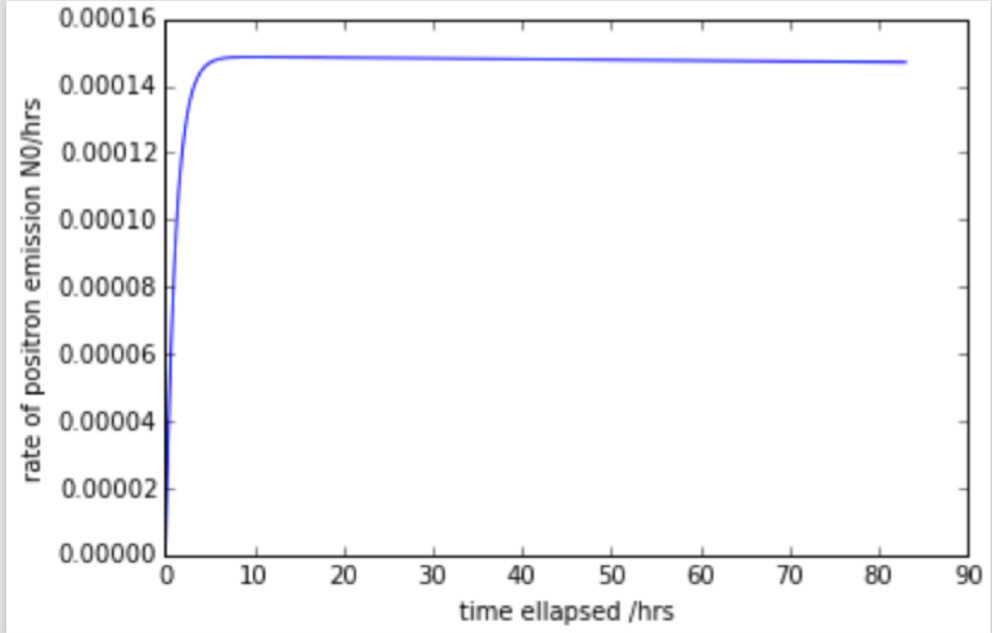
\includegraphics{Figures/C2F1}
\decoRule
\caption[C2F1]{The activity of the 68Ge/68Ga fuel as function of time. The units of y axis is the number of initial 68Ge atoms.}
\label{fig:C2F1}
\end{figure}

The ten hours that the sample takes to reach its full activity allows a reasonable time to transfer the sample from the point of production to the point of use. Transportation is required, since the production of 68Ge is a nuclear reaction and particle accelerators and nuclear sources are needed for its production. The activity drops to 90\% of its maximum roughly a month after it has reached it. Based on cost efficiency and other circumstances, such as safety, the slow rate of this decay in activity allows to choose a convenient period of time of the order of a month over which the sample has to be replaced by a new one in order to keep the activity high enough so stimulated emission is still possible (see below).

There are other, more complex ways of creating polarised positrons. These methods are costly and do not result in a significant raise in polarisation. They use circularly polarised $\gamma$ ray radiation for electron-positron pair creation. Two of these methods are the $\gamma$ ray radiation from helical ondulators and the use of Compton scattering. Appendix A contains an estimate on how much radioactive source is needed to be able to create a burst of 1kJ $\gamma$-ray laser. 

\section{Fuel Production}

There are many ways for producing 68Ge some of them are listed below:

\begin{equation}
\label{e4}
Ga^{nat} + \rho = Ge_{68} + xn
\end{equation}

\begin{equation}
\label{e5}
Ge^{nat} + \rho = Ge_{68} + p + xn
\end{equation}

\begin{equation}
\label{e6}
Zn^{nat} + \alpha = Ge_{68} + xn
\end{equation}

For 68Ge production simply the elementary form of each source is used disregarding the actual isotope content, hence the number of neutrons emitted during the reaction depends on the actual isotope that is struck by the incoming particle ($\rho$ or $\alpha$).
The actual reactions summarised in Fig. 2.1 and Fig. 2.2 [2]:

\begin{figure}[h]
\centering
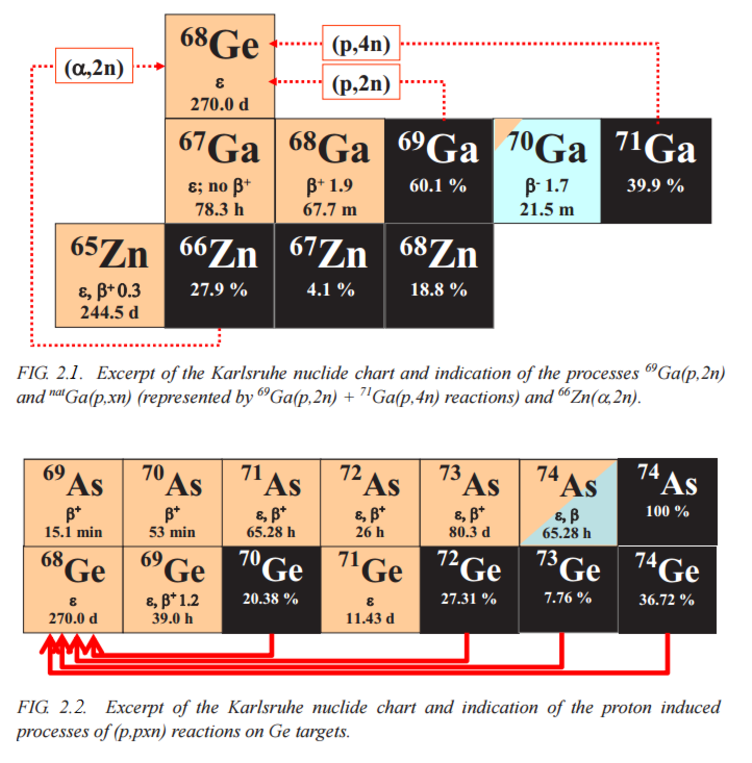
\includegraphics{Figures/C2F2}
\decoRule
\caption[C2F2]{Summarised Reactions}
\label{fig:C2F2}
\end{figure}

\begin{figure}[h]
\centering
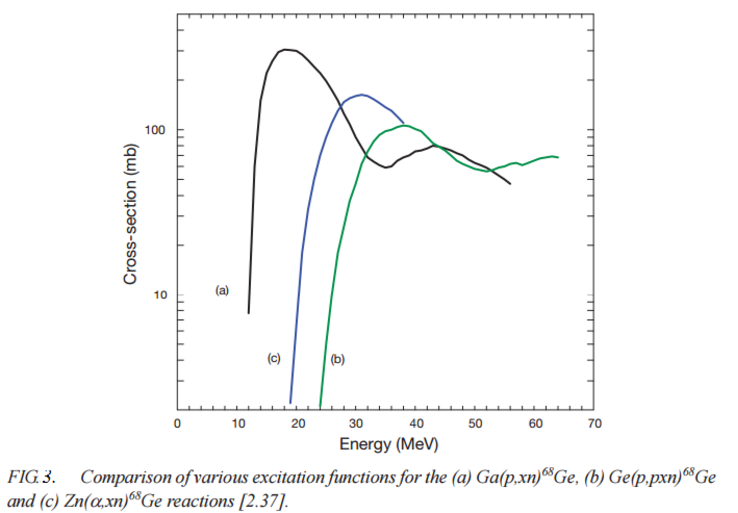
\includegraphics{Figures/C2F3}
\decoRule
\caption[C2F3]{Cross sections of each production paths against the energy of the projected incoming particle [2]}
\label{fig:C2F3}
\end{figure}

As the curves show, the best way to acquire is to use a Gallium source bombarded with protons of approximately 18MeV energy. This range of energy is easily achievable in many accelerators. For the Gallium reaction, the first maximum corresponds for a maximum in the partial cross section of the 69Ga(p,2n)68Ge reaction and the second local maximum corresponds to a peak in the partial cross section of the 71Ga(p,4n)68Ge. 

\section{Accumulation of Positrons}

The accumulation of a large number of positrons that are ready to be released in ultrashort pulses is essential in the creation of a $\gamma$-ray laser. Since the overall efficiency of the whole process is very low, i.e. most of the positrons radiated by the source will not participate in the stimulated emission, the more positrons available at the time of usage of the laser, the more likely that stimulated annihilation is achievable and also the more energy the output laser pulse will have. Most accumulation instruments comprise of an ultrapure neon moderator, a trap and an accumulator. The purpose of the neon moderator is to slow down the positrons to a few eV once it has left the source and radially compressed via the rotating wall technique. These slow positrons are then transported to a trap where they are radially confined. However, in order to prevent positrons returning to the moderator when transferred to the trap the moderator potential must be gradually increased at a steady rate.

\section{The Penning-Malmberg Trap}

One way to store positrons for a longer period of time is the use of the so called Penning-Malmberg trap (PM trap) [3]. There are many advantages of employing a PM trap, most importantly it is the long confinement times that allow the accumulation of large amounts of positron particles. Other advantages include: the potential for brightness enhancement by compressing the positron plasma and the ability to generate short positron pulses.
The main features of the PM trap is a strong axial magnetic field that confines the particles radially and a quadrupole field for axial confinement. An improved version of it is the multi-cell trap (MCT).Positrons can be stored for very long times in a plasma state with this device and also can be cooled and released in tailored bursts. The main challenge to overcome is the increasing space charge density upon accumulation that degrades confinement. 
To successfully trap the positrons an energy loss mechanism is required, the most common technique is the use of a buffer gas, which exploits inelastic scattering collisions between the particles. A lower electrostatic potential and gas pressure is obtained through the use of electrodes of increasing radii. The positrons when first passing through the trap are subject to a high gas pressure so that there are a greater number of collisions between the positrons. As the positrons progress through the higher stages they continue to collide with one another and the pressure of the buffer-gas is progressively reduced. This causes the temperature of the positrons to reduce down to room temperature in approximately 0.1 s. The most effective gas for this purpose is Nitrogen. At most 30\% of incoming positrons are trapped in the accumulator. Utilising this three stage buffer-gas trap enables the accumulation of several hundred million positrons with lifetimes of several minutes. 4x109 positrons have been confined at 1.2 K where the gas pressure is estimated to be less than or equal to 8x10-17 mbar [4].
Although there are alternative methods to using a buffer-gas, however, they are far less efficient. Such techniques are dependent upon the positron sources utilised, for example, to make use of the pulsed nature of a linac-based positron source the potential on one of the end caps is reduced allowing the positron pulse to enter the trap and then increasing the potential thus preventing the pulse from escaping. However, for our purposes the use of a buffer-gas is the most ideal. However, the one drawback from the use of a buffer-gas is that the gas molecules allow annihilation to occur thus reducing the storage time.
The aim here is to accumulate a large number of positron particles which are then delivered in pulses at a later time. Consequently, the critical issue of positron loss as a result of transport and annihilation must be considered. During a collision the wavefunctions of the positron and electron overlap causing them to annihilate. However, if a vacuum of good quality is used this is not a significant issue. Therefore, an ultra-high vacuum (UHV) environment is required to prevent annihilation. Alternatively we can reduce the loss of positrons by removing any grease, oil or other small quantities of large molecules from the system as otherwise positrons can attach themselves to these molecules, thus resulting in much higher rates of annihilation. Additionally, positron loss as a result of transportation is due to a torque exerted on the plasma due to the presence of any external force; the effect of this exerted torque is that it causes the plasma to expand radially. The viscous drag experienced by the plasma as a result of not only the collisions with the neutrally charged background gas but also the asymmetries of the trap caused by machining imperfections are examples of sources of such a torque.
In the multi-cell configuration, the plasma is divided into m parts, hence for a given confining potential, m times more particles can be stored. The positrons coming from the source are first compressed with the rotating wall technique[5]. The typical strength of magnetic fields used is approximately 5 T. The graphical design for the MCT is shown on Fig. 4.[6]

\begin{figure}[h]
\centering
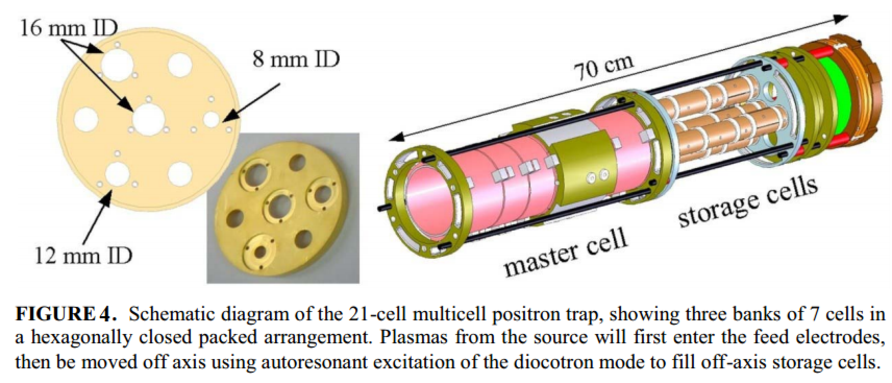
\includegraphics{Figures/C2F4}
\decoRule
\caption[C2F4]{Diagram of Multicell Positron Trap}
\label{fig:C2F4}
\end{figure}

This technique has been implemented to confine 109 particles for a time duration longer than a day [7]. The positrons are ejected from the trap in pulses. If parabolic potential is rapidly applied on an ensemble of positrons, they arrive at the target at roughly the same time and positron pulses with width of approximately 15-20ns can be created that contains over 106 particles. In order to lower the pulse width, a buncher is also introduced between the accumulator and the target. After introducing the buncher, the pulses are improved to have a width of approximately 1ns with a number of 70x106 positrons. The created positron plasmas have an areal density of typically 109 cm-2, which is still low for most of the Positronium interaction wished to be observed later. In order to produce the exotic Positronium atoms, subnanosecond pulses of positrons with a minimum density of 1x10'10 cm-2 [8] are required. For this reason the sample is further compressed by a pulsed magnetic field. The resulting density is in the range of (2-4) x 10'10 cm'-2.
The maximum number of positrons that can be stored in the MCT increases with the confining potential and the tube length of the cells. Fig. 5. shows the results of the experiment done by Danielson et al. on storing positrons.

\begin{figure}[h]
\centering
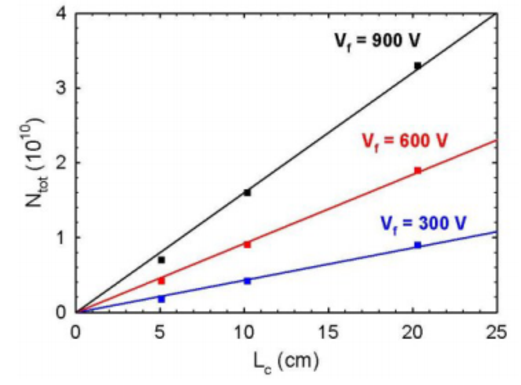
\includegraphics{Figures/C2F5}
\decoRule
\caption[C2F5]{The number of stored positrons as a function of the length of tubes used in the multicell conifguration for three different trapping voltages.}
\label{fig:C2F5}
\end{figure}

If it is assumed that 1 in every 1000 accumulated positrons will participate in the stimulated emission, the number of positrons need to be stored is in the order of 10'19 for achieving a pulse of gamma ray laser with an energy of 1 kJ. If the linear relationship between the stored positrons and cell length is assumed to be held for all cell length, for a trapping voltage of 900V a tube of length 62500km is required. Even if 1000 tubes are used, every one of them has to be 62.5km long that is equivalent to a circular tube with radius of 10km. Just for comparison, this is more than twice as long as the LHC at CERN. 
`	The length of the cells could be lowered significantly if higher trapping voltages were available, however raising the voltage can lead to a few complications. For example, higher voltages will result in heating that lowers the stability of the positron plasma due to the formation of Ps with the background neutral gas. 


\section{Decoupled Surko-Trap}

The areal density requirements for the positron pulses mentioned above are not only met but exceeded via the use of a decoupled Surko-trap, which is able to emit a beam of intense positrons of areal densities exceeding 3 x 10'10 cm-2   [8] in subnanosecond pulses. The Surko-type and the Penning-Malmberg trap share a lot of common features, for clarity purposes these are pointed out once more in the description for the Surko-trap below. Advantages of employing this variation of a Surko trap include the longer lifetimes of positrons and the cost reduction due to removing the need for large and expensive magnets and vacuum chambers.
From Fig. 6. [8] it can be seen that the decoupled Surko-trap of an approximate length of 5.5m consists of a positron source, a trap, an accumulator, a target chamber and a buncher. Positrons once leaving the source are subject to an ultrapure neon moderator, the purpose of this is to slow the positrons down to a few eV. However, the exposure of the moderator to the nitrogen buffer gas results in the beam intensity to be greatly reduced to approximately 4 x 10'6 e'+ s'(-1)  [8]. An axial magnetic field is then used to radially confine the positrons, and the presence of the electrostatic potential well confines the particles along the direction of the magnetic field.

\begin{figure}[h]
\centering
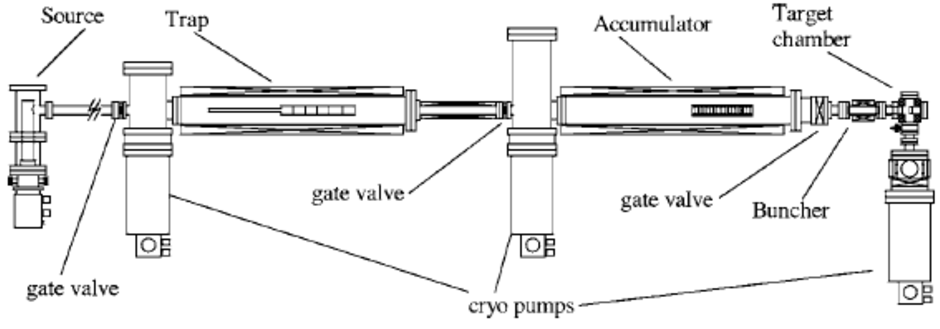
\includegraphics{Figures/C2F6}
\decoRule
\caption[C2F6]{Schematic diagram of the composition of all the components of the decoupled Surko-trap.}
\label{fig:C2F6}
\end{figure}

The positrons then enter a two-stage Surko-type trap infused with a buffer gas, as can be seen in Fig. 7. Stage 1 consists of a narrow electrode with an inside diameter of 8mm and stages 2a and 2b contains a segmented electrode with inside diameter 2.54cm, which allows the radial compression of positrons in stage 2b via a ‘rotating wall’ electric field. The positron cloud can be compressed to a final diameter of approximately 1.3mm full width at half maximum, where the rf is 5MHz, when a cooling gas (SF6 or CF4) [9]of a pressure of 20\% of that of the Nitrogen buffer gas is introduced. There is no significant loss in the lifetime of the positrons as a result of introducing a cooling gas [8].  
Stage 1 contains the Nitrogen buffer gas with an approximate pressure of 1x10'-3 Torr; the pressure of the gas is progressively reduced in stages 2a and 2b to an order of magnitude less than in stage 1, noting that there is very little difference in pressure across 2a and 2b. The lifetime of positrons are approximately 2s, and as a result of the short lifetime, the trap operates at 4Hz to maximise the number of particles passing through the trap. The efficiency of trapping using this particular method is approximately 20\% [8].

\begin{figure}[h]
\centering
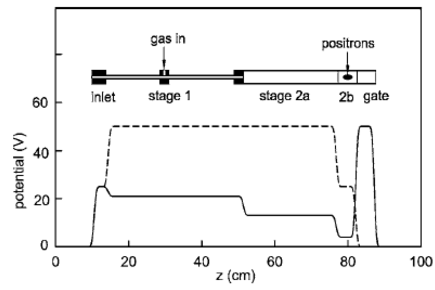
\includegraphics{Figures/C2F7}
\decoRule
\caption[C2F7]{Electrode structure of the buffer gas trap. The solid and dashed lines represent the potentials required for the trapping and releasing of positrons.}
\label{fig:C2F7}
\end{figure}

The positrons are then transferred to the accumulator and are trapped within a harmonic potential well. The positron loss is very low when the next pulse of positrons are transferred into the accumulator. As a result of cross-field transport, positrons have a typical lifetime of approximately 100s within the accumulator, however, this mechanism of positron loss has been eliminated via the ‘rotating wall’ technique.
The rotating wall in addition to counteracting the outward transport of the plasma, compresses the plasma. However, the plasma heats up as it is compressed, therefore a cooling mechanism, in the form of a cooling gas (SF6 or CF4) is needed at a pressure where there is no significant increase in the positron annihilation rate. The frequency of the rotating wall is approximately 4MHz and for a few seconds is then raised to 8MHz, thus allowing a containment of up to 95x10'6 positrons.
Using the techniques described the plasma areal densities achieved at the target are up to 2x10'-9 cm -2, however, the areal density can be further increased to (2-4) x 10'10 cm'-2 with the use of a pulsed magnetic field of approximately 1T which is applied at the target.
The plasma is transported from the accumulator using a parabolic potential which is able to eject the positrons at the same time, thus producing pulses of positrons which are restricted to a width of 15-20ns containing more than 1x10'6 positrons. Subnanosecond pulses are achieved with the application of a buncher, the structure of which can be seen in Fig. 8.[8] The buncher is positioned just before the positrons reach the target and is able to compress a maximum of 70x10'6 positrons into approximately a 1ns pulse [8].

\begin{figure}[h]
\centering
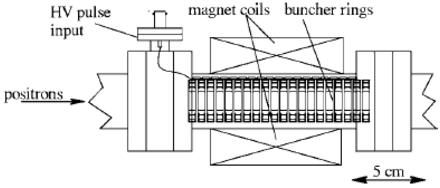
\includegraphics{Figures/C2F8}
\decoRule
\caption[C2F8]{Schematic diagram showing the structure of the buncher.}
\label{fig:C2F8}
\end{figure}

The use of a multiring accelerator enables the acceleration of the beam to approximately5kV, whilst eliminating additional positron losses as well as the associated gamma ray bursts.
To reiterate, the aim here is to accumulate a large number of positron particles which are then delivered in pulses at a later time. Consequently, the critical issue of positron loss as a result of transport and annihilation must be considered. We can take measures to reduce the loss of positrons by removing any grease, oil or other small quantities of large molecules from the system as otherwise positrons can attach themselves to these molecules, thus resulting in much higher rates of annihilation. Additionally, positron loss as a result of transportation is due to a torque exerted on the plasma in the presence of any external force; the effect of this exerted torque is that it causes the plasma to expand radially. The viscous drag experienced by the plasma as a result of not only the collisions with the neutrally charged background gas but also the asymmetries of the trap caused by machining imperfections are examples of sources of such a torque. [10]
The decoupled Surko-trap described is able to create 1ns pulses of approximately 60x10'6 low energy positrons, with areal densities of 3x10'10 cm-2. [8] However, in order to fulfil the final objective of creating a gamma-ray laser we require a mechanism of trapping a relatively greater magnitude of positrons than discussed above. Methods of rescaling the Surko trap can be considered to allow a larger quantity of positrons to be trapped. The rescaling has proved to be a limitation of the decoupled Surko trap; if it were to be scaled longitudinally it would produce plasmas that were long and thin and ultimately unstable. The idea of the multi cell configuration applied on the decoupled Surko-type trap could significantly raise the numbers achieved in positron accumulation.


\section{Beam Control}
The next objective after the accumulator is the tailoring of a positron beam that will provide suitable initial conditions within the silicon target to enable stimulated annihilation of a BEC sometime after impact. In particular the beam will need to reach a certain areal density, be of a sufficiently low temporal width, contain a large enough positron population and be sufficiently polarised. The polarisation of the beam will have already been set before beam extraction as will the total positron population, but the amount of positrons lost between the accumulator and the target will depend on the techniques used. Developments have been made on this subject by the group of D.B. Cassidy, the main features of the technique are described in [8].

The first of interest is the properties of the beam just after leaving the trap, and how these properties can be controlled. They are set by the techniques used to extract the stored positrons in the accumulator. The most effective way to get an intense pulse of positrons is to quickly switch the potential of the electric field within the accumulator from the harmonic confining potential to a parabolic shape in order to achieve longitudinal compression. This will force all the positrons forward in one very short pulse. This must be done in the smallest possible time period as to create a pulse that is temporally narrow as possible. The pulse in its original form after extraction can have a temporal width of around 15–20 ns [8], as has been achieved experimentally. To further compress this width, the beam will be first guided through the buncher apparatus where a pulsed voltage is applied in such a way as to create a harmonic like potential extremely rapidly. This forces the beam to further compress to subnanosecond scales of around 1ns [8]. The rise time of the pulse is very small compared to the pre buncher pulse width of the beam.

\section{Formation of Positronium Atoms and Molecules}

If an intense positron beam is incident of porous silica, Positronium molecule formation can be observed. Silica is used because of its low cost and because it is an insulator. Metals and semiconductors cannot be used due to the high number of free electrons their screening effect prohibits Ps formation. [Ps formation] Positrons interact with the electrons in the bulk of the material and form Positronium (Ps) atoms. Up to 40\% of incoming positrons can be transformed to Ps [11]. These atoms have a lifetime of <1ns within the material. However if it is made porous, the atoms can diffuse into the voids of the material, significantly raising their lifetimes.

The vacuum lifetime of Ps depends on its spin state. If it’s a singlet (called para-positronium, pPs) the lifetime is very short (125ps), hence atoms created in the singlet state decay technically immediately after formation. The triplet state (known as ortho-positronium, oPs) has a lifetime of 142ns that allows enough time for Ps-Ps interaction.  The overall probability of two atoms interacting is about 10\% [The production of molecular Ps]. These interaction can result in one the two outcomes:

\begin{equation}
\label{e7}
oPs + oPs = pPs +pPs
\end{equation}

\begin{equation}
\label{e8}
X+oPs+oPs=X+Ps2
\end{equation}

The former is called spin exchange quenching (SEQ) and the second is the molecular positronium formation.
Eventually all the positrons of the incident beam annihilate with the electrons of the material. There is a pulse of $\gamma$ rays immediately after the sample is irradiated by the positron beam coming from direct annihilation and the fast decay of pPs molecules.	After Ps-Ps interaction, annihilation takes place immediately since these mechanisms essentially turn long-lived triplet states into either pPs (SEQ) or molecular positronium (Ps2) that also annihilates technically immediately. Raising the incoming positron beam intensity hence lowers the lifetime of Ps atoms.

At room temperature, the molecule formation is approximately ten times more likely than SEQ that is hence a secondary process, however at higher temperature molecule formation is suppressed and SEQ becomes more significant. Also, as a study shows [12], the ratio of the different types of quenching depends on the geometrical structure of the target silica bulk. If the voids within the target material is randomly distributed molecule formation is enhanced, while if they are aligned in one particular dimension, SEQ is more likely. As temperature is increased in the first type of geometry, quenching is suppressed. This can be explained by the surface state of Ps. As temperature is increased, Ps atoms desorb from the surface and there is a lack of third body that is needed for molecule formation and lack of phonons needed for quenching in order to conserve energy. For the first geometry the discrete levels of the surface states cannot accommodate for the hyperfine structure (no SEQ) and if the temperature is high enough (no surface Ps, hence no Ps2 formation) there is no significant quenching. In the second geometry, there are no surface states due to the continuous levels in energy and thus quenching is temperature independent and can be considered entirely due to SEQ [13].

In order to create a Bose-Einstein Condensate (BEC) all sorts of quenching should be eliminated. For this purpose the size of the voids should be small enough so SEQ is suppressed and the temperature of the walls should be relatively high (room temperature or higher) so Ps atoms desorb from the surfaces and molecule formation is avoided. In order to achieve BEC a high density of particles is needed and hence the created Ps atoms should be collected somewhere within the material. Increased quenching effects due to the increased density should also be taken into account.

 
% Chapter Template

\chapter{An Antimatter Bose-Einstein Condensate} % Main chapter title

\label{Chapter3} % Change X to a consecutive number; for referencing this chapter elsewhere, use \ref{ChapterX}

%----------------------------------------------------------------------------------------
%	SECTION 1
%----------------------------------------------------------------------------------------

\section{Main Section 1}

Lorem ipsum dolor sit amet, consectetur adipiscing elit. Aliquam ultricies lacinia euismod. Nam tempus risus in dolor rhoncus in interdum enim tincidunt. Donec vel nunc neque. In condimentum ullamcorper quam non consequat. Fusce sagittis tempor feugiat. Fusce magna erat, molestie eu convallis ut, tempus sed arcu. Quisque molestie, ante a tincidunt ullamcorper, sapien enim dignissim lacus, in semper nibh erat lobortis purus. Integer dapibus ligula ac risus convallis pellentesque.

%-----------------------------------
%	SUBSECTION 1
%-----------------------------------
\subsection{Subsection 1}

Nunc posuere quam at lectus tristique eu ultrices augue venenatis. Vestibulum ante ipsum primis in faucibus orci luctus et ultrices posuere cubilia Curae; Aliquam erat volutpat. Vivamus sodales tortor eget quam adipiscing in vulputate ante ullamcorper. Sed eros ante, lacinia et sollicitudin et, aliquam sit amet augue. In hac habitasse platea dictumst.

%-----------------------------------
%	SUBSECTION 2
%-----------------------------------

\subsection{Subsection 2}
Morbi rutrum odio eget arcu adipiscing sodales. Aenean et purus a est pulvinar pellentesque. Cras in elit neque, quis varius elit. Phasellus fringilla, nibh eu tempus venenatis, dolor elit posuere quam, quis adipiscing urna leo nec orci. Sed nec nulla auctor odio aliquet consequat. Ut nec nulla in ante ullamcorper aliquam at sed dolor. Phasellus fermentum magna in augue gravida cursus. Cras sed pretium lorem. Pellentesque eget ornare odio. Proin accumsan, massa viverra cursus pharetra, ipsum nisi lobortis velit, a malesuada dolor lorem eu neque.

%----------------------------------------------------------------------------------------
%	SECTION 2
%----------------------------------------------------------------------------------------

\section{Main Section 2}

Sed ullamcorper quam eu nisl interdum at interdum enim egestas. Aliquam placerat justo sed lectus lobortis ut porta nisl porttitor. Vestibulum mi dolor, lacinia molestie gravida at, tempus vitae ligula. Donec eget quam sapien, in viverra eros. Donec pellentesque justo a massa fringilla non vestibulum metus vestibulum. Vestibulum in orci quis felis tempor lacinia. Vivamus ornare ultrices facilisis. Ut hendrerit volutpat vulputate. Morbi condimentum venenatis augue, id porta ipsum vulputate in. Curabitur luctus tempus justo. Vestibulum risus lectus, adipiscing nec condimentum quis, condimentum nec nisl. Aliquam dictum sagittis velit sed iaculis. Morbi tristique augue sit amet nulla pulvinar id facilisis ligula mollis. Nam elit libero, tincidunt ut aliquam at, molestie in quam. Aenean rhoncus vehicula hendrerit.
% Chapter Template

\chapter{Gamma Ray Laser: Gamma Ray Optics} % Main chapter title

\label{Chapter4} % Change X to a consecutive number; for referencing this chapter elsewhere, use \ref{ChapterX}

%----------------------------------------------------------------------------------------
%	SECTION 1
%----------------------------------------------------------------------------------------

\section{A Summary of $\gamma$-ray Optics}

The construction of a $\gamma$-ray laser requires development in the field of  $\gamma$-ray optics. This is essential for two significant reasons. Firstly, once stimulated annihilation has taken place, the resulting $\gamma$-rays will be emitted in multiple random directions. This entails the requirement of either the reflection or refraction of said $\gamma$-rays to prevent the loss of  ~50$\%$ of the energy of the laser. If this refraction of the rays has then taken place, there will then be at least two independent beams of $\gamma$-rays which will then need to be made coherent to prevent destructive interference which could contribute to another large loss of power of the laser. Finally, a lens will be required to allow for the focussing of the laser to allow for more precise targeting and to prevent dispersion of the beam over a wide area.The difficulties of $\gamma$-ray optics arise due to the inherent properties of $\gamma$-rays. $\gamma$-rays are highly energetic and possess a small wavelength which therefore means that they would normally pass through the space between atoms of most materials, thereby indicating that reflection and refraction via conventional mirrors and prisms is not possible. However contemporary research into this area has demonstrated that, for high energy $\gamma$-rays, there may be a ‘significant’ level of refraction which could be useful in the production of a $\gamma$-ray laser. 

%-----------------------------------
%	SUBSECTION 1
%-----------------------------------
\section{Theory of $\gamma$-ray Optics}

The refraction or reflection of $\gamma$-rays, as with any electromagnetic radiation, is dependent on the index of refraction of the material being used to conduct said process. The refractive index is dependent on the energy of the incident radiation and is described in \ref{e1}, 
\begin{equation}
\label{e1}
n(E) = 1 - \delta(E)-i\beta(E)
\end{equation}
where the imaginary part describes absorption whilst the real part describes the refraction. The Fresnel equations, as shown in equations \ref{e2} and \ref{e3} where p refers to parallel polarisation and s refers to normal polarisation, then dictate that reflection also depends on the refractive index. 
\begin{equation}
\label{e2}
r_p =\frac{n^2\sin\alpha-\sqrt{(n^2-\cos^2\alpha)}}{n^2\sin\alpha+\sqrt{(n^2-\cos^2\alpha)}}
\end{equation}
\begin{equation}
\label{e3}
r_s =\frac{\sin\alpha-\sqrt{(n^2-\cos^2\alpha)}}{\sin\alpha+\sqrt{(n^2-\cos^2\alpha)}}
\end{equation}
Using the Fresnel equations, the reflectivity for a surface can be determined by taking the modulus of \ref{e2} and \ref{e3}, where light polarised in differing directions will have differing reflectivity.  For low energy radiation, for example in the optical spectrum, the real part of \ref{e1} is greater than unity, allowing for easy design of refractive materials and mirrors for these frequencies. However as the wavelength of the incident radiation decreases (as the energy increases), the reflectivity at the normal ($\alpha$ = $90^o$) decreases rapidly. This is especially the case for high energy radiation such as X-Ray and $\gamma$. However by applying Snell’s law we can determine that the refraction angle as measured from the normal to the surface will be greater than $90^o$ if the condition in \ref{e4} is satisfied:
\begin{equation}
\label{e4}
n_r = 1 - \delta < 1
\end{equation}
which is the same as saying that total internal reflection takes place when t where tis the critical angle and can be determined using \ref{e5}:
\begin{equation}
\label{e5}
\cos\alpha_t = 1 - \delta \textrm{ or } \alpha_t = \sqrt{2\delta} \textrm{ if } \delta<<1
\end{equation}
\newline
\newline
The previous equations describe the mathematics of a grazing incidence telescope which essentially uses reflection from curved surfaces to focus light. The value of $\delta$ can also be roughly estimated using \ref{e6}:
\begin{equation}
\label{e6}
\delta = -2.7 \frac{\rho Z \lambda^2}{A}
\end{equation}
where $Z$ and $A$ are the atomic number and atomic weight respectively, and $\rho$ is the density of the material. It can clearly be seen that $\delta$ decreases rapidly with increasing energy , converging towards $0$. The focal length of an array of lenses is dependent on $\delta$ via the relation given in \ref{e7}:
\begin{equation}
\label{e7}
f=\frac{R}{2 \delta N}
\end{equation}
where $R$ is the radius of curvature of the concave lens and $N$ is the number of lenses in use. For X-Rays, a reasonable focal length is attainable via the use of hundreds of lenses.

%-----------------------------------
%	SUBSECTION 2
%-----------------------------------

\section{Development of $\gamma$-ray Optics}
The area of $\gamma$ ray optics is still continuously under research and is currently being developed from the area of  X-Ray optics. X-Ray optics is also an area under research, however lenses and reflective processes are in existence for X-Rays. There is currently one “hard” energy X-Ray mirror in operation in the Nuclear Spectroscopic Telescope Array that operates in an energy range of 3-79 KeV(reference The Nuclear Spectroscopic telescope array (NuSTAR) High energy X-Ray mission). This X-Ray mirror is based on the Wolter I design which uses the previously described grazing incidence principle to image distant objects. The principle used is from equation \ref{e7} where multiple glass optics coated in multiple layers of metal (e.g gold) at different depths to provide a suitable focal length with an increased field of view. The reason for the depth grading of the multilayer optics is to increase the grazing angle of the incident radiation. 
\newline
\newline
Previous findings for $\gamma$-rays had originally implied that $\delta$ from \ref{e1} was always negative for high energy radiation. However a recent paper has demonstrated that, if the energy of the $\gamma$ radiation is greater than $0.7 MeV$, then $\delta$ changes sign which leads to $n$ being greater than 1. By using Silicon prisms, refraction on the order of $10^{-9}m$ was achieved with $\gamma$-rays of energy up to $2 MeV$. This refraction was verified by the measurement of a parallel beam travelling through air below the beam travelling through the prism. These findings are explained via Delbruck scattering, where the photon directly interacts with the electric field of the nucleus of the incident atom, causing virtual pair-production to take place. The photon is then re-scattered by this virtual pair. In principle, these findings could be used to develop refractive Silicon prisms. Further study also needs to be undertaken to investigate the use of higher $Z$ materials such as gold as a rudimentary calculation indicates a $\delta$ value of $3\times10^{-5}$ in the energy range of $1 MeV$. A lens with this property has a theoretical focal length of $3m$ and could be used to focus the $\gamma$-rays produced by the annihilation laser for focussed usage.
\newline 
\newline
Although it is not possible to reflect the $\gamma$-rays, a beam of the desired energy can be achieved through the annihilation of double the amount of Ps, which in itself presents its own challenges. Notably, it will also increase the amount of shielding required in the reverse direction of the beam and it will also require a substantially larger amount of positrons to be produced. There have been advancements in the material that can be used for shielding. The most common material used is lead, which is convenient as it is both cheap and easily available. Lead provides shielding which is approx $20-30\%$ better than other materials such as soil, though more exotic materials such as depleted uranium and lead foams have demonstrated a much greater ability to absorb $\gamma$-rays. There are also some novel lightweight shielding materials made from aluminium that can be used. However, in terms of cost effectiveness, lead remains the most economic material. 
\newline
\newline
In terms of $\gamma$-rays, shielding can be easily accomplished via the use of lead plates with a thickness on the order of ~4 inches. \ref{e8} was used to determine the thickness necessary for attenuation using lead:
\begin{equation}
\label{e8}
I_x = I_0 \exp(-\mu x)
\end{equation}
where $I_x$ is the intensity of the photon after attenuation, $I_0$ is the initial energy of the photon, $\mu$ is the Linear Attenuation Coefficient of Lead for the specified initial energy, and $x$ is the thickness of material needed for the required level of attenuation. This level of shielding will lead to a $90\%$ attenuation of $\gamma$-rays at the specified energy level. However in order to ensure that the risk of irradiation is low, the thickness of lead shielding is doubled to 4 inches. For convenience, rather than using a 4 inch solid plate of lead around the room, lead plates of 0.5 inches would instead be used. This then acts as a cost saving mechanism because, once the outer plate has begun to deteriorate due to continuous exposure, it can then be removed and disposed of, exposing the next level of plating. An additional plate can then be added at the rear of the plating wall. It should be noted however that the shielding required is not limited to shielding $\gamma$-rays. There will be high energy $e^+$ particles that will miss the Silica target, and are therefore free to impact the surrounding walls of the room, therefore leading to the creation of Bremsstrahlung radiation. This electromagnetic radiation is created when charged particles are deflected by other charged particles, and will occur in this case if the $e^+$ particles are deflected by a positively charged nucleus. In order to shield against this radiation, it is preferable to use a low $Z$ element. It was determined that the most convenient material to use would be liquid water. The convenience of this is clear as water can easily be pumped out and replaced. To provide complete shielding the layout would be a wall of lead surrounding the equipment, then a pipe containing a sufficient amount of water (a pipe with a diameter of ~6 inches), with a final wall of lead plating after the pipe. The reasoning behind this was to ensure that the first wall of lead would shield against any $\gamma$-rays that are emitted in the wrong direction and so cannot be used in the lasing process. The water layer would then shield against any Bremsstrahlung radiation that is generated. Finally the outer layer of lead would then shield against any electromagnetic radiation of high energy that may be produced due to the Bremsstrahlung radiation and to prevent any final leakage of $\gamma$-rays.
 
% Chapter Template

\chapter{Gamma Ray Laser: Unresolved Problems} % Main chapter title

\label{Chapter5} % Change X to a consecutive number; for referencing this chapter elsewhere, use \ref{ChapterX}

%----------------------------------------------------------------------------------------
%	SECTION 1
%----------------------------------------------------------------------------------------

\section{Summary}

Although a design has been proposed which should in principle produce the desired $\gamma$-ray laser, there are a number of issues at all stages of the process that must be resolved before the design can be implemented in practice. These are given by the part of the process they pertain to.

%-----------------------------------
%	SUBSECTION 1
%-----------------------------------
\section{Positrons}

Of the positrons that will be produced most will be lost before they can produce Positronium. The positron beam produced has a width that is $1.3mm$ (approximately). In comparison the cavity itself will be about $0.1\mu m$. Assuming a silica target of the order of $1\mu m$, the vast majority of the positrons will never strike the target and thus will be unable to produce positrons. This is further compounded by the limitations on the number of positrons that can be trapped. At this point $10^7$ can be kept. To counter this there will need to be further work into the use of multiple or combined trapping mechanisms.
\newline
\newline
After reaching the target, most of the remaining positrons will either annihilate with an electron in the target, or will form para-Positronium (lifespan around $120 ns$), although as shown beforehand aerogel limits the losses to $60\%$.
\newline
\newline
The critical temperature for BEC formation is dependent on the density of the ortho-Positronium atoms to the $2/3$ power. Thus it is desirable to raise the density of the positrons so as to increase that of the Positronium and thus increase the critical temperature. If this can be achieved, then the time required for cooling the Positronium will be reduced and less will have decayed before a BEC can be formed and annihilation stimulated.
%-----------------------------------
%	SUBSECTION 2
%-----------------------------------

\section{Materials}
There remains a great uncertainty over the choice and use of a material which will provide not only the target for the positron beam but the means by which Positronium will be produced and the cavity where it will be cooled and annihilated. The key issues are:
\begin{itemize}
	\item   Pore density, size and distribution: The optimal configuration to prevent spin quenching is to have small, randomly distributed pores. If too many pores are produced however this will lead to an unequal distribution in the Positronium atoms and will not allow a sufficient density to be reached in many of the cavities, thus effectively losing more Positronium without further laser production.
	\item Pore shape: In a spherical pore, there is no preferred direction for the annihilation and thus $\gamma$-rays will be emitted equally in every direction. To limit this the intention is to produce pores which are longer, and perhaps narrower. This increases the Positronium along the desired axis and thus the laser will be more intense along this direction.
	\item Manufacturing process: Although a certain configuration of pores is desired, it is not yet known how this could be achieved.
	\item Paramagnetic defects: Unpaired electrons will be induced to oscillate by the UV cooling lasers, producing magnetic fields. These will affect the incoming positrons and the Positronium atoms moving through to the cavity, in a manner that will result in the loss of many. Thus it is desirable to find a material which is not subject to these.
	\item Target resilience: Bombardment by protons could cause substantial damage to the structure of the target. This will affect the rate at which Positronium can be successfully produced, so the useful lifetime of the target must be ascertained.
	\item Premature annihilation: Certain materials (e.g. carbon nanotubes) suffer from causing annihilation on their surfaces or within. The desired material must not be the cause of such a problem if it is to be of use.
\end{itemize}
%----------------------------------------------------------------------------------------
%	SECTION 2
%----------------------------------------------------------------------------------------

\section{Cooling}
Problems pertaining to this are closely related to the materials, and also affect the ability to form a BEC at a given density. It is desirable to find a method to cool the Positronium as far as possible.
\begin{itemize}
	\item Target Temperature: In order to suppress Ps2 formation (and the premature accompanying annihilation), the target must be kept hot, $300K$ may suffice but this must be ascertained. This will affect the rate at which cooling can occur by effectively eliminating the thermalisation process. The laser will itself be wholly dependent on laser cooling.
	\item Positronium lifetime: Even with thermalisation, Positronium will not survive for a sufficient time to be cooled to a BEC in its ground state. Using UV lasers the Positronium can be excited from the 1s to 2p states which can double or even triple the lifetime (Lifetime of 2p ~ $3.2ns$ but this ‘resets’ the lifetime of the 1s post decay. Excitations can occur more than once).
	\item Laser induced paramagnetism: As discussed before, a material must be found that will not be subject to this.
\end{itemize}

\section{Stimulated Annihilation}
To induce annihilation a low energy IR pulse will be sent which will change the spin state of the ortho-Positronium to para-Positronium. The wavelength will need to be known and apparatus assembled to produce said pulse. It is also not known how much of the Positronium will change spin states as a result. The duration must be short enough so as not to emerge (and interfere) with the laser.
Although elongation of the pores may increase the intensity along a preferred axis, a method to further induce emission along said axis will need to be found so as to increase the intensity of the laser and reduce the shielding required.
\newline
\newline
In order to conserve momentum, each annihilation will result in two photons travelling in opposite directions. Either a way to use both should be found, or shielding will be required to prevent damage/injury that would result from the unwanted beam.
 
% Chapter Template

\chapter{Gamma Ray Laser: Possible Applications} % Main chapter title

\label{Chapter4} % Change X to a consecutive number; for referencing this chapter elsewhere, use \ref{ChapterX}

%----------------------------------------------------------------------------------------
%	SECTION 1
%----------------------------------------------------------------------------------------

\section{Main Section 1}

Lorem ipsum dolor sit amet, consectetur adipiscing elit. Aliquam ultricies lacinia euismod. Nam tempus risus in dolor rhoncus in interdum enim tincidunt. Donec vel nunc neque. In condimentum ullamcorper quam non consequat. Fusce sagittis tempor feugiat. Fusce magna erat, molestie eu convallis ut, tempus sed arcu. Quisque molestie, ante a tincidunt ullamcorper, sapien enim dignissim lacus, in semper nibh erat lobortis purus. Integer dapibus ligula ac risus convallis pellentesque.

%-----------------------------------
%	SUBSECTION 1
%-----------------------------------
\subsection{Subsection 1}

Nunc posuere quam at lectus tristique eu ultrices augue venenatis. Vestibulum ante ipsum primis in faucibus orci luctus et ultrices posuere cubilia Curae; Aliquam erat volutpat. Vivamus sodales tortor eget quam adipiscing in vulputate ante ullamcorper. Sed eros ante, lacinia et sollicitudin et, aliquam sit amet augue. In hac habitasse platea dictumst.

%-----------------------------------
%	SUBSECTION 2
%-----------------------------------

\subsection{Subsection 2}
Morbi rutrum odio eget arcu adipiscing sodales. Aenean et purus a est pulvinar pellentesque. Cras in elit neque, quis varius elit. Phasellus fringilla, nibh eu tempus venenatis, dolor elit posuere quam, quis adipiscing urna leo nec orci. Sed nec nulla auctor odio aliquet consequat. Ut nec nulla in ante ullamcorper aliquam at sed dolor. Phasellus fermentum magna in augue gravida cursus. Cras sed pretium lorem. Pellentesque eget ornare odio. Proin accumsan, massa viverra cursus pharetra, ipsum nisi lobortis velit, a malesuada dolor lorem eu neque.

%----------------------------------------------------------------------------------------
%	SECTION 2
%----------------------------------------------------------------------------------------

\section{Main Section 2}

Sed ullamcorper quam eu nisl interdum at interdum enim egestas. Aliquam placerat justo sed lectus lobortis ut porta nisl porttitor. Vestibulum mi dolor, lacinia molestie gravida at, tempus vitae ligula. Donec eget quam sapien, in viverra eros. Donec pellentesque justo a massa fringilla non vestibulum metus vestibulum. Vestibulum in orci quis felis tempor lacinia. Vivamus ornare ultrices facilisis. Ut hendrerit volutpat vulputate. Morbi condimentum venenatis augue, id porta ipsum vulputate in. Curabitur luctus tempus justo. Vestibulum risus lectus, adipiscing nec condimentum quis, condimentum nec nisl. Aliquam dictum sagittis velit sed iaculis. Morbi tristique augue sit amet nulla pulvinar id facilisis ligula mollis. Nam elit libero, tincidunt ut aliquam at, molestie in quam. Aenean rhoncus vehicula hendrerit.
% Chapter Template

\chapter{Gamma Ray Laser: Construction Cost and Time Scale} % Main chapter title

\label{Chapter5} % Change X to a consecutive number; for referencing this chapter elsewhere, use \ref{ChapterX}

%----------------------------------------------------------------------------------------
%	SECTION 1
%----------------------------------------------------------------------------------------

\section{Main Section 1}

Lorem ipsum dolor sit amet, consectetur adipiscing elit. Aliquam ultricies lacinia euismod. Nam tempus risus in dolor rhoncus in interdum enim tincidunt. Donec vel nunc neque. In condimentum ullamcorper quam non consequat. Fusce sagittis tempor feugiat. Fusce magna erat, molestie eu convallis ut, tempus sed arcu. Quisque molestie, ante a tincidunt ullamcorper, sapien enim dignissim lacus, in semper nibh erat lobortis purus. Integer dapibus ligula ac risus convallis pellentesque.

%-----------------------------------
%	SUBSECTION 1
%-----------------------------------
\subsection{Subsection 1}

Nunc posuere quam at lectus tristique eu ultrices augue venenatis. Vestibulum ante ipsum primis in faucibus orci luctus et ultrices posuere cubilia Curae; Aliquam erat volutpat. Vivamus sodales tortor eget quam adipiscing in vulputate ante ullamcorper. Sed eros ante, lacinia et sollicitudin et, aliquam sit amet augue. In hac habitasse platea dictumst.

%-----------------------------------
%	SUBSECTION 2
%-----------------------------------

\subsection{Subsection 2}
Morbi rutrum odio eget arcu adipiscing sodales. Aenean et purus a est pulvinar pellentesque. Cras in elit neque, quis varius elit. Phasellus fringilla, nibh eu tempus venenatis, dolor elit posuere quam, quis adipiscing urna leo nec orci. Sed nec nulla auctor odio aliquet consequat. Ut nec nulla in ante ullamcorper aliquam at sed dolor. Phasellus fermentum magna in augue gravida cursus. Cras sed pretium lorem. Pellentesque eget ornare odio. Proin accumsan, massa viverra cursus pharetra, ipsum nisi lobortis velit, a malesuada dolor lorem eu neque.

%----------------------------------------------------------------------------------------
%	SECTION 2
%----------------------------------------------------------------------------------------

\section{Main Section 2}

Sed ullamcorper quam eu nisl interdum at interdum enim egestas. Aliquam placerat justo sed lectus lobortis ut porta nisl porttitor. Vestibulum mi dolor, lacinia molestie gravida at, tempus vitae ligula. Donec eget quam sapien, in viverra eros. Donec pellentesque justo a massa fringilla non vestibulum metus vestibulum. Vestibulum in orci quis felis tempor lacinia. Vivamus ornare ultrices facilisis. Ut hendrerit volutpat vulputate. Morbi condimentum venenatis augue, id porta ipsum vulputate in. Curabitur luctus tempus justo. Vestibulum risus lectus, adipiscing nec condimentum quis, condimentum nec nisl. Aliquam dictum sagittis velit sed iaculis. Morbi tristique augue sit amet nulla pulvinar id facilisis ligula mollis. Nam elit libero, tincidunt ut aliquam at, molestie in quam. Aenean rhoncus vehicula hendrerit.
% Chapter Template

\chapter{Gamma Ray Laser: An Alternative Method} % Main chapter title

\label{Chapter6} % Change X to a consecutive number; for referencing this chapter elsewhere, use \ref{ChapterX}

%----------------------------------------------------------------------------------------
%	SECTION 1
%----------------------------------------------------------------------------------------

\section{Summary}
One of the significant issues with the previous design is accumulating enough Positrons to create sufficient Positronium which can then be used to reach the critical density required ($1.2\times 101^{19} cm^3$) to form a Bose-Einstein condensate. The number of Positrons needed is not currently attainable with any Positron beam that is in functional use at the present time. The previous section of unresolved problems describes these issues and the issues that cannot be solved following the lack of Positrons in great detail. Here we describe a method which may be feasible with current technology which does not involve the use of a Positronium Bose-Einstein condensate, and instead involves the use of a free electron laser. 

%-----------------------------------
%	SUBSECTION 1
%-----------------------------------
\section{An Alternative}
The alternative method involves the use of relativistic bound states of electron-positron bound states rather than the requirement for slow Positronium presented in the previous method. These bound states are more easily produced at relativistic energies which are easily reached in the current generation of particle accelerators available. In this schema various methods can be used. The seemingly most feasible method is to fire $\gamma$-rays at high density slabs of material which will then cause pair production to take place. However the main issue with a method like this is the lack of efficiency (similar to issues in the previous schema) which leads to a large loss of Positrons. Current efficiencies for Positron-Electron pair collection is on the order of $10\%$. In order to then cool the $e^+e^-$ pairs to ensure Positron production, a device known as the “Kayak-Paddle Cooler” (KPC) can be used. 
\newline
\newline
A schematic of a KPC device is shown in the figure below. The device uses magnetic fields and RF cavities to sufficiently cool the incoming beam of $e^+e^-$  pairs to provide the correct conditions to allow for the formation of Positronium. The reason for this is that, for Positronium formation to take place, quantum processes need to become dominant which means that the beams need to be brought down to sub-relativistic energies. The magnetic wigglers and RF Cavities are used in an alternating fashion to ensure maximum cooling is achieved. Magnetic wigglers are a magnetic setup of parallel magnets with alternating north and south poles which cause the oscillation of the charged particles within the field. The reason this method can be used to cool is because charged particles moving in such a way in an applied field will cause the emission of synchrotron radiation. These photons will then carry energy away causing a reduction in temperature of said charged particles. The radiofrequency (RF) cavity will then be used to further cool the charged particles via ionisation cooling. RF cavities are normally used for the acceleration of charged particles, however they can be produced in such an arrangement to cause cooling rather than heating. They are also used to cause the bunching of particles passing through the cavity at varying energies. An RF cavity is essentially a metallic chamber which contains within it an electromagnetic field. A generator provides electromagnetic waves which will then become resonant and will build up within the cavity. The resonance at which these waves build up is dependent on the size and shape of the cavity and is specifically calibrated for the particles that will be entering the cavity. The RF cavity is designed such that particles travelling through with a specified energy will not “see” the electromagnetic field permeating the cavity, therefore meaning that these particles will be unaffected. However particles with energy either greater than or less than this energy will be accelerated or decelerated respectively, leading to the bunching of particles. This will also cause the particles energy to be adjusted accordingly, leading to the majority of particles possessing an energy near the ideal energy required to allow the bound state of Positronium to form. A key  factor affecting the efficient running of an RF cavity is that they must be kept in a superconducting state to prevent the loss of energy to electrical resistance. In order to ensure this the metal surrounding the cavity and the generator can be cooled using liquid nitrogen thereby ensuring that they function as superconductors.    
\newline
\newline
The above method in normal usage would produce incoherent $\gamma$-rays. However it can be modified to allow for the generation of a coherent beam of $\gamma$-rays in addition to Positronium atoms. The first main modification is to introduce two counter propagating lasers along the axis of the $e^-e^+$ beam. These two laser beams will act as an undulator for the charged particles. The system will also be tuned such that the radiation emitted in the frame of reference of the charged particles is equal to the ionisation energy of Positronium. This leads to stimulated formation of Positronium via energy loss once the particles emit said radiation. This also acts as a further cooling process within the system.  
\newline
\newline
As has been previously mentioned, oPs will annihilate to produce 3 $\gamma$-photons. In the reference frame of the beam, these photons will have parameterised energy as shown in \ref{8.1}, \ref{8.2}, \ref{8.3}:
\begin{equation}
\label{8.1}
\hbar \omega = \chi m c^2
\end{equation}
\begin{equation}
\label{8.2}
\hbar \omega_1 = (1+ \eta_1)m c^2
\end{equation}
\begin{equation}
\label{8.3}
\hbar \omega_2 = (1+\eta_2)m c^2
\end{equation}
where $\omega$, $omega_1$, and $\omega_2$  refers to the angular frequency of each photon respectively and $\eta$ and $\chi$ are parameters (Note: $mc^2\simeq0.511 MeV$and $e_I=mc^26.77 eV$). The conservation laws for energy and momentum in the frame of the beam then dictate that:
\begin{equation}
\label{8.4}
\chi + \eta_2 +\eta_2 = \frac{v^2}{c^2} - \epsilon
\end{equation}
\begin{equation}
\label{8.5}
\chi \hat{k} + (1+\eta_1)\hat{k_1} + (1+\eta_2)\hat{k_2} = 2\frac{\vec{v}}{c}
\end{equation}
where the unit vectors denote the associated vectors of the emitted photons. In this schema it is assumed that the energy of one of the emitted photons is negligible. We can then take $\chi << 1$ which then, using momentum conservation, leads us to the conclusion that $\eta_1,\eta_2 << 1$. This then allows us to determine that the hard photons will be emitted in almost opposite directions, with a separation from the normal of the direction of the particle beam of a small angle. With this in mind we can then set $\hat{k_2}=-\hat{k_1}+\hat{\delta}$, and because $v^2 << c^2$, and $\epsilon \simeq10^{-5}$:
\begin{equation}
\label{8.6}
\mid \vec{\delta} \mid = \mid \frac{2 \frac{\vec{v}}{c} - \chi \hat{k} - (\eta_1 -\eta_2\hat{k_1})}{(1+\eta_2)} \mid<<1
\end{equation}
The result from \ref{8.6} proves that the emitted photons will be in opposite directions within a cone of aperture that is less than 1 (in the rest frame of the Ps). For this to work it is a necessity that the photons that co-propagate with the electrons have energy equivalent to the Positronium ionisation energy in the rest frame of the electrons. This condition allows for a derivation of the relativistic factor of the electron and positron beams which is given by:
\begin{equation}
\label{8.7}
\gamma_p \simeq \frac{\epsilon^*}{\epsilon}
\end{equation}
where $\epsilon^*$ is the rest energy of the co-propagating photons in their reference frame and has been previously defined. As the undulator photons need to be resonant with the spontaneously scattered photons, we can derive a relation between the undulator wavelength and that of the co-propagating photons which then allows us to determine that the undulator could be provided by a microwave beam and the stimulating laser can be provided by an FEL operating at a wavelength of $0.5\AA$. The final step in this schema is to then introduce stimulated annihilation of the formed positronium atoms. 
\newline
\newline
The spontaneous emission of a soft photon in the energy interval and solid angle is given by \ref{8.8}:
\begin{equation}
\label{8.8}
W_{sp} = \frac{f(\chi)\Delta\chi\Delta\Omega}{A \tau 4 \pi}
\end{equation}
where the function $f(\chi)$ refers to the spectral distribution calculated by blah shown in figure blah, $A$ is a normalisation factor and $\tau$ is the life span of the positronium. As there is a stimulating electromagnetic field present, the annihilation rate is then proportional to the number of photons present in the mode associated with the energy transition. A ratio can then be calculated for the number of stimulated against the number of spontaneously emitted photons. This ratio can then be evaluated and leads to the determination that the probability of a stimulated event taking place is on the order of $10\%$. The number of stimulated photons produced can then be calculated which is also dependent on the number of positronium atoms. 
\newline
\newline
The whole schema described has a procedural time essentially dependent on two factors; the cooling time of the beams and the lifetime of the positronium atoms. The cooling time can be determined to be on the order of a few tens of seconds using standard parameters in equation blah.
\newline
\newline
This method is potentially feasible with current technology and will allow for the production of a coherent beam of $\gamma$-rays, however explicit power calculations have not been carried out so the laser may not provide the $1kJ$ required. Also no focussing technology currently exists which is still an issue for fine targeting with the beam.

% Chapter Template

\chapter{Final Remarks} % Main chapter title

\label{Chapter7} % Change X to a consecutive number; for referencing this chapter elsewhere, use \ref{ChapterX}

%----------------------------------------------------------------------------------------
%	SECTION 1
%----------------------------------------------------------------------------------------

\section{Main Section 1}

Lorem ipsum dolor sit amet, consectetur adipiscing elit. Aliquam ultricies lacinia euismod. Nam tempus risus in dolor rhoncus in interdum enim tincidunt. Donec vel nunc neque. In condimentum ullamcorper quam non consequat. Fusce sagittis tempor feugiat. Fusce magna erat, molestie eu convallis ut, tempus sed arcu. Quisque molestie, ante a tincidunt ullamcorper, sapien enim dignissim lacus, in semper nibh erat lobortis purus. Integer dapibus ligula ac risus convallis pellentesque.

%-----------------------------------
%	SUBSECTION 1
%-----------------------------------
\subsection{Subsection 1}

Nunc posuere quam at lectus tristique eu ultrices augue venenatis. Vestibulum ante ipsum primis in faucibus orci luctus et ultrices posuere cubilia Curae; Aliquam erat volutpat. Vivamus sodales tortor eget quam adipiscing in vulputate ante ullamcorper. Sed eros ante, lacinia et sollicitudin et, aliquam sit amet augue. In hac habitasse platea dictumst.

%-----------------------------------
%	SUBSECTION 2
%-----------------------------------

\subsection{Subsection 2}
Morbi rutrum odio eget arcu adipiscing sodales. Aenean et purus a est pulvinar pellentesque. Cras in elit neque, quis varius elit. Phasellus fringilla, nibh eu tempus venenatis, dolor elit posuere quam, quis adipiscing urna leo nec orci. Sed nec nulla auctor odio aliquet consequat. Ut nec nulla in ante ullamcorper aliquam at sed dolor. Phasellus fermentum magna in augue gravida cursus. Cras sed pretium lorem. Pellentesque eget ornare odio. Proin accumsan, massa viverra cursus pharetra, ipsum nisi lobortis velit, a malesuada dolor lorem eu neque.

%----------------------------------------------------------------------------------------
%	SECTION 2
%----------------------------------------------------------------------------------------

\section{Main Section 2}

Sed ullamcorper quam eu nisl interdum at interdum enim egestas. Aliquam placerat justo sed lectus lobortis ut porta nisl porttitor. Vestibulum mi dolor, lacinia molestie gravida at, tempus vitae ligula. Donec eget quam sapien, in viverra eros. Donec pellentesque justo a massa fringilla non vestibulum metus vestibulum. Vestibulum in orci quis felis tempor lacinia. Vivamus ornare ultrices facilisis. Ut hendrerit volutpat vulputate. Morbi condimentum venenatis augue, id porta ipsum vulputate in. Curabitur luctus tempus justo. Vestibulum risus lectus, adipiscing nec condimentum quis, condimentum nec nisl. Aliquam dictum sagittis velit sed iaculis. Morbi tristique augue sit amet nulla pulvinar id facilisis ligula mollis. Nam elit libero, tincidunt ut aliquam at, molestie in quam. Aenean rhoncus vehicula hendrerit.

%----------------------------------------------------------------------------------------
%	THESIS CONTENT - APPENDICES
%----------------------------------------------------------------------------------------

\appendix % Cue to tell LaTeX that the following "chapters" are Appendices

% Include the appendices of the thesis as separate files from the Appendices folder
% Uncomment the lines as you write the Appendices

% Appendix A

\chapter{References} % Main appendix title

\label{AppendixA} % For referencing this appendix elsewhere, use \ref{AppendixA}

Chapter 2

%% Appendix A

\chapter{Appendices Description: Supporting Evidence of the Project Development} % Main appendix title

\label{AppendixB} % For referencing this appendix elsewhere, use \ref{AppendixA}

Write your Appendix content here.
%% Appendix A

\chapter{Project Milestone Plan} % Main appendix title

\label{AppendixC} % For referencing this appendix elsewhere, use \ref{AppendixA}

Add Gantt Chart and Development Description.
%% Appendix A

\chapter{Formal Debrief of Project Meetings} % Main appendix title

\label{AppendixA} % For referencing this appendix elsewhere, use \ref{AppendixA}

Include Summary, Agendas and Minutes
%% Appendix A

\chapter{Assessment} % Main appendix title

\label{AppendixE} % For referencing this appendix elsewhere, use \ref{AppendixA}

Include description, mid term assessment, self assessment and open letter to board

%----------------------------------------------------------------------------------------
%	BIBLIOGRAPHY
%----------------------------------------------------------------------------------------

\printbibliography[heading=bibintoc]

%----------------------------------------------------------------------------------------

\end{document}  
